\newpage
\subsection{Interfaces}
    
    \subsubsection{Tableau des scores}
    Pendant le déroulement du jeu, le joueur a besoin de connaitre certaines informations concernant son personnage, la partie et les autres joueurs. 
    Pour fournir ces informations, nous avons opté pour un tableau des scores disponible à n’importe quel moment de la partie. Ce tableau permet également un classement simple, clair et rapide des joueurs en fonction de leurs points.
    La difficulté principale de ce tableau des scores est la synchronisation entre un script coté client qui doit actualiser à chaque pression de la touche TAB le score ainsi que la présence de chaque joueur et la récupération des données de chaque Player, mises à jour en temps réel sur le serveur.
    
    \begin{figure}[hbt!]
            \centering
            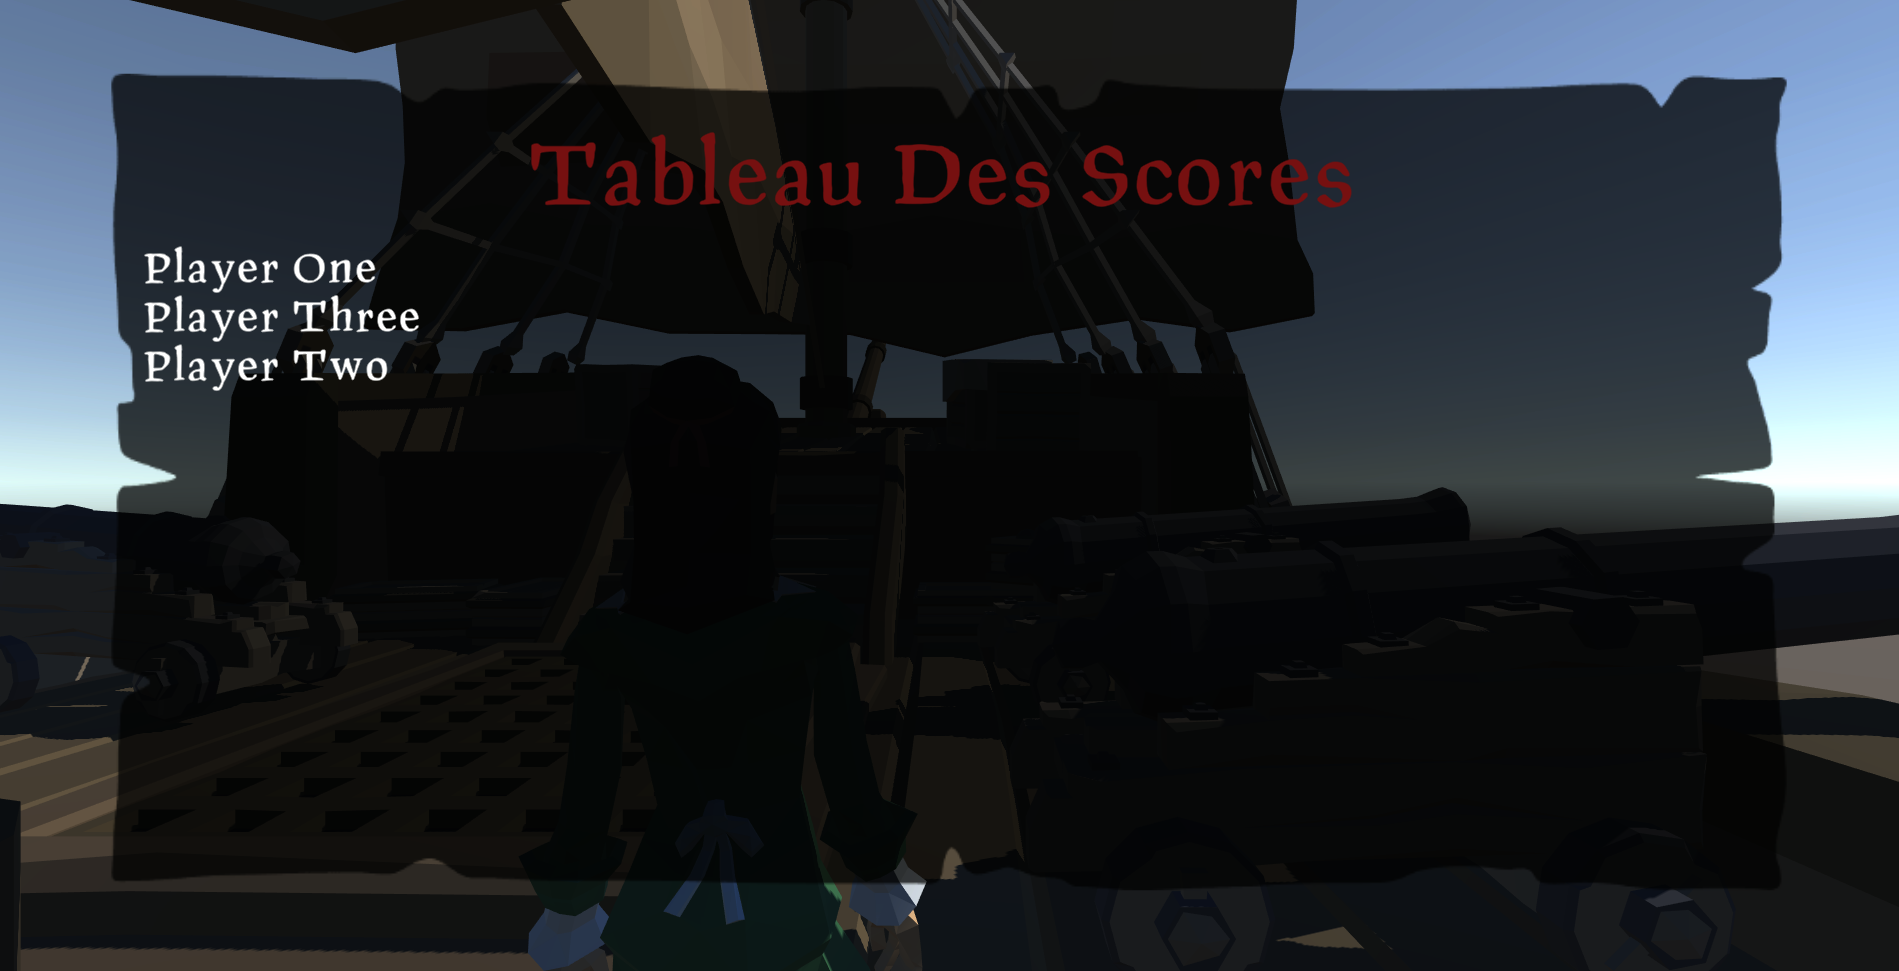
\includegraphics[scale=0.3]{img/scoreboard.PNG}
            \caption{Première version du tableau des scores}
    \end{figure}
    
    \subsubsection{Système de chat}
    